\documentclass[output=paper]{../langscibook}
\ChapterDOI{10.5281/zenodo.4449774}
\author{Emel Kucukali\affiliation{Marmara University}\orcid{}}
\title{Multilingual teachers, plurilingual approach and L3 acquisition:  Interviews with multilingual teachers and their L3/L3+ students}
\abstract{The article reports a study on plurilingual approaches (PA) of three multilingual teachers in three foreign language classrooms (English, German and Russian) at a Turkish state university. The qualitative study explored the attitudes of multilingual teachers to PA and the response of their L3/L3+ students ($N=5$) to the plurilingual practices in class. The perceptions of participants were investigated from the holistic paradigm in multilingualism. Data were collected through interviews and graphic elicitation tasks. Data were analyzed through content and visual-based analysis. The results indicated three main themes based on participants’ perceptions of PA:
(1) implementation,
(2) benefits to learning and
(3) the role of multilingual teachers in L3 Acquisition. Both teachers and students displayed positive attitudes in findings (1) and (2). However, participants’ perceptions were not homogeneous in finding (3), which revealed some issues. The overall findings suggest that multilingual teachers should play a crucial role in plurilingual and L3 classrooms in a Turkish context.
% \keywords{L3 \& L3+ learners, multilingual teachers, plurilingual approach, third language acquisition}
}
\IfFileExists{../localcommands.tex}{
  \addbibresource{../localbibliography.bib}
  % add all extra packages you need to load to this file

\usepackage{tabularx,multicol}
\usepackage{url}
\urlstyle{same}

\usepackage{enumitem}

\usepackage{pifont}

\usepackage{listings}
\lstset{basicstyle=\ttfamily,tabsize=2,breaklines=true}

\usepackage{./langsci-optional}
\usepackage{./langsci-lgr}
\usepackage{./langsci-gb4e}

\usepackage{langsci-plots} 

\makeatletter
\let\pgfmathModX=\pgfmathMod@
\usepackage{pgfplots,pgfplotstable}%
\let\pgfmathMod@=\pgfmathModX
\makeatother

\usepackage{siunitx}
\sisetup{output-decimal-marker={.},detect-weight=true, detect-family=true, detect-all, input-symbols={\%}, free-standing-units,table-align-text-pre=false,group-digits=false,detect-inline-weight=math}
\DeclareSIUnit[number-unit-product={}]{\percent}{\%}
\makeatletter \def\new@fontshape{} \makeatother
\robustify\bfseries % For detect weight to work

\usepackage{todonotes}

  \newcommand*{\orcid}{}

\renewcommand{\lsChapterFooterSize}{\footnotesize}

\makeatletter
\let\thetitle\@title
\let\theauthor\@author
\makeatother

\newcommand{\togglepaper}[1][0]{
%   \bibliography{../localbibliography}
  \papernote{\scriptsize\normalfont
    \theauthor.
    \thetitle.
    To appear in:
    Jorge Pinto \& Nélia Alexandre (eds.),
    Multilingualism and third language acquisition: Learning and teaching trends.
    Berlin: Language Science Press. [preliminary page numbering]
    }
  \pagenumbering{roman}
  \setcounter{chapter}{#1}
  \addtocounter{chapter}{-1}
}


 
  %% hyphenation points for line breaks
%% Normally, automatic hyphenation in LaTeX is very good
%% If a word is mis-hyphenated, add it to this file
%%
%% add information to TeX file before \begin{document} with:
%% %% hyphenation points for line breaks
%% Normally, automatic hyphenation in LaTeX is very good
%% If a word is mis-hyphenated, add it to this file
%%
%% add information to TeX file before \begin{document} with:
%% %% hyphenation points for line breaks
%% Normally, automatic hyphenation in LaTeX is very good
%% If a word is mis-hyphenated, add it to this file
%%
%% add information to TeX file before \begin{document} with:
%% \include{localhyphenation}
\hyphenation{
affri-ca-te
affri-ca-tes
au-ton-o-mous
Cha-basse
Din-ger-fel-der
plu-ri-lin-gual
Ya-na-pra-sart
Mi-ri-ci
Ström-quist
}

\hyphenation{
affri-ca-te
affri-ca-tes
au-ton-o-mous
Cha-basse
Din-ger-fel-der
plu-ri-lin-gual
Ya-na-pra-sart
Mi-ri-ci
Ström-quist
}

\hyphenation{
affri-ca-te
affri-ca-tes
au-ton-o-mous
Cha-basse
Din-ger-fel-der
plu-ri-lin-gual
Ya-na-pra-sart
Mi-ri-ci
Ström-quist
}
 
  \togglepaper[4]%%chapternumber
}{}

\shorttitlerunninghead{Multilingual teachers, plurilingual approach and L3 acquisition}%%use this for an abridged title in the page headers
\begin{document}
\maketitle


\section{Introduction}


With the increase of immigration and globalization, multilingualism has attracted the attention of language researchers and educators (\citealt{CenozGenesee1998}; \citealt{Jessner1999}; \citealt{Cenoz2013a}). Research on multilingualism has created a new multilingual perspective which adopts a holistic philosophy and considers all the individual’s languages as an integrated whole (\citealt{Cook1992}; \citealt{Grosjean2008}; \citealt{Cenoz2013a}). In addition, the multilingual perspective distinguishes between how monolinguals and bi-\slash multilinguals learn languages or between L2 learners and L3/L3+ learners \citep{Hufeisen2004}. This classification resulted in new pedagogical applications some of which are called plurilingual approaches (\citealt{CouncilOfEurope2001}; \citealt{Cenoz2013a,Cenoz2013b}; \citealt{Otwinowska2014}). Plurilingual approaches (PA hereafter) challenge the isolation of languages, focus on learners' plurilingual repertoires and promote the integration and diversity of languages in the classroom (\citealt{BeaccoEtAl2010}).

As a pedagogy, PA are built on a holistic view on multilingualism (\citealt{Grosjean2008}; \citealt{Cenoz2013a,Cenoz2013b}) and are suggested as a practice in multilingual education \citep{Cenoz2009}. Therefore, research on PA focuses mostly on learners and schools in bi- and multilingual contexts of immigrant and minority communities (\citealt{Cenoz2013b}; \citealt{GarciaLi2014}). For this reason, more research is suggested on PA in different contexts with a different type of students (\citealt{Cenoz2013a,Cenoz2013b}; \citealt{CenozGorter2017}). Furthermore, teachers and their language repertoire are defined as a significant variable in multilingual education \citep{Cenoz2009}. That is why research on multilingual teachers and the influence of their languages on their teaching is also recommended \citep{Ellis2013}. Moreover, research in the Turkish context is not enough to give a picture of PA, third language acquisition (TLA) and multilingual teachers in Turkish education. With an attempt to give light to these issues, the present study will focus on PA of three multilingual teachers in three foreign languages (FL hereafter) classrooms at a Turkish state university. The aim of the study is to explore the attitudes of multilingual teachers to PA and the response of their L3/L3+ students to plurilingual practices in class through a qualitative perspective.~


\section{Literature review}


\subsection{Holistic view on multilingualism}



One of the generic definitions of multilingualism is “the command and\slash or use of two or more languages by the respective speaker” (\citealt{HerdinaJessner2002}: 52). However, apart from the generic definitions above, multilingualism could be approached from two different philosophies. They are challenging each other and are called the \emph{holistic} (multilingual) and the \emph{monolingual} view on multilingualism \citep{Grosjean2008}. While the monolingual view claims that multilinguals are the sum of multiple separate monolinguals, the multilingual view proposes that multilinguals have a unique language system of multi-competencies. {Furthermore}, the multilingual view suggests that multilinguals differ with regard to language-related cognitive processing because their multi-competencies are integrated and domain-specific (\citealt{Cook1993}; \citealt{Grosjean2008}). Depending on the interlocutors or domain, multilinguals may shuttle between mono-, bi-, tri- or quadrilingual speech modes along a situational continuum. In the monolingual mode, bilinguals speak to monolinguals in either of their languages, while in the multilingual speech mode they speak to multilingual interlocutors by mixing multiple languages in the form of code-switching \citep{Grosjean2008}.



\subsection{Third language acquisition vs. second language acquisition}



The literature adopting a holistic view on multilingualism proposes that there is a difference between second language acquisition (SLA) and TLA (\citealt{Jessner1999}; \citealt{HerdinaJessner2002}; \citealt{Hufeisen2004}; \citealt{MarxHufeisen2004}; \citealt{Cenoz2013a,Cenoz2013b}).

The factor model \citep{Hufeisen2004} explains the difference between SLA and TLA with the cognitive leap between the learning of the first (L2) and the second foreign language (L3). L3 learners learn differently from L2 learners because the former have the cognitive and linguistic experience of learning another foreign language during SLA. After their experience with the first foreign language (L2), L3 learners have upgraded to a significantly higher metalinguistic and metacognitive level. The following stages of learning the subsequent languages (L3+) also contribute to cognitive leaps afterwards but with little significance.  In other words, while there is little cognitive distinction between L3 and L3+ learners, the gap between L2 and L3 learners is crucial due to a significant cognitive transformation between SLA and TLA \citep{Hufeisen2004}.

Similarly, \citet{Cenoz2013b} suggests that TLA is different from SLA because L3 learners reactivate and relate all their languages and adapt strategies to TLA from previous learning experiences. SLA focuses on the learning of a specific language in separation, while bilingualism, multilingualism, and TLA are unified under the umbrella of involving the additional languages of multilinguals in the learning process (\citealt{CenozGorter2011}).



\subsection{Plurilingual approaches}



The holistic paradigm in multilingualism has been realized in education as pedagogical applications called plurilingual approaches (PA) \citep{CouncilOfEurope2001,BeaccoEtAl2010,Cenoz2013a}. PA challenge isolation of languages and promote the integration and diversity of languages in the classroom because languages support and contribute to each other to build up a flexible and dynamic competence. Therefore, plurilingual approaches focus on learners' plurilingual and intercultural repertoires, raise learners’ language awareness and give equal value to all languages and cultures \citep{BeaccoEtAl2010}. The Council of Europe has already promoted PA in education to meet the diverse and democratic character of the European population (\citealt{CouncilOfEurope2001}; \citealt{BeaccoEtAl2010}).

PA are defined as “making use of the learners’ first and other languages to teach more effectively” \citep[102]{Otwinowska2014}. They cover pedagogies such as alternation of languages, conscious cross-linguistic comparison and transfer, metalinguistic awareness strategies, code-switching and using cognates (\citealt{CouncilOfEurope2001}; \citealt{BeaccoEtAl2010}; \citealt{HerdinaJessner2002}; \citealt{HufeisenNeuner2004}; \citealt{Cenoz2013b};  \citealt{JessnerEtAl2016}).  \citet{Otwinowska2014} also suggests the using of English as a bridge between learners’ native language and their other languages by making use of similarities for better language learning.



\subsection{Learners’ metalinguistic awareness and teachers’ plurilingual awareness}



Metalinguistic and cross-linguistic awareness are properties of a multilinguals'\linebreak metasystem which involves “specific meta-skills” (\citealt{HerdinaJessner2002}: 129). These meta-skills contribute to the bi- and multilinguals’ cognitive system and give them an advantage over monolinguals in language learning. Metalinguistic\linebreak awareness “refers to the ability to focus attention on language as an object in itself or to think abstractly about language and, consequently, to play with or manipulate language” \citep[42]{Jessner2006}. Cross-linguistic awareness is defined as the awareness of the relationships between languages \citep[116]{Jessner2006}.

Teachers’ plurilingual awareness is more compounded than that of learners and refers to “the complex ability to promote plurilingual approaches in the language classroom” \citep[103]{Otwinowska2014}. Teachers’ plurilingual awareness has three main components: cross-linguistic and metalinguistic awareness of similarities and differences between the language taught and the learners’ L1, L2 and L3/L3+; knowledge about adopting a plurilingual approach in the classroom, which refers to training learners to search for similarities across the languages they know; psycholinguistic knowledge of individual learner differences that facilitate learning such as, knowing that bilingual learners differ from multilinguals in the process of language learning \citep{Otwinowska2014}.



\subsection{Previous research}



Research on PA in TLA is conducted mainly in plurilingual, minority and immigrant contexts. It focuses mostly on the learners but less on the teachers and even less on both of them.

Research on learners covers the benefits of PA and prior language knowledge on L3 learning. The positive effects of PA include raising learners’ metalinguistic awareness \citep{JessnerEtAl2016} and facilitating language learning (\citealt{BonoStratilaki2009}). These benefits are enhanced when the school languages are also used in social interactions in family and community or in school contexts which promote plurilingual practices and cross-linguistic strategies (\citealt{BonoStratilaki2009}). Similarly, learners’ prior language knowledge has a positive effect on third language learning both in plurilingual (\citealt{BonoStratilaki2009}; \citealt{Cenoz2013b}; \citealt{Sanchez2015}) and formal instruction contexts (\citealt{Kemp2001}; \citealt{GibsonHufeisen2003};  \citealt{DeAngelis2007}). In addition, \citet{Dmitrenko2017} found a significant correlation between the learners’ degree of multilingualism and the use of multilingual strategies of language learning. The main difference between L2 and L3/L3+ learners was the preference of cross-linguistic strategies \citep{Dmitrenko2017}.

Research on multilingual teachers and PA is little but valuable. It indicates that multilingual teachers have higher plurilingual awareness \citep{Otwinowska2014} and higher metalinguistic awareness (\citealt{Ellis2004,Ellis2013}) than their bi- and monolingual counterparts. On the one hand, compared to monolingual ones, multilingual teachers of English as a Second Language (ESL) in Australia are more likely to adopt cross-linguistic practices in their classrooms (\citealt{Ellis2004,Ellis2013}; \citealt{HigginsPonte2017}) such as using knowledge of other languages at the level of phonology, lexis, grammar, syntax, discourse, and pragmatics to understand the target language and help students with their challenges (\citealt{Ellis2004,Ellis2013}). On the other hand, teachers in some European contexts have positive attitudes towards PA (\citealt{GrivaEtAl2016}) but make little use of plurilingual strategies in L3 teaching classes (\citealt{GöbelVieluf2014}).

In one of the few studies (\citealt{AroninOLaoire2003}) in the field of TLA regarding students and their teachers, the findings indicate that trilingual students from Israel and Ireland prefer their teachers of L3 to be trilingual as well even if the teacher only teaches one language. Trilingual students prefer their trilingual teachers to use the three languages of the classroom for facilitating and practical reasons (\citealt{AroninOLaoire2003}).

Research on TLA, PA and multilingual teachers in Turkish contexts is very scarce. There have been initiatives to integrate plurilingualism in education \citep{Mirici2008}, however Turkish instructors of English reported no familiarity with or training concerning plurilingualism \citep{Celik2013}. In terms of TLA and L3 learners, \citet{Korkmaz2013} found that English Language Teaching (ELT) university students used their L2 (English) to make a lexical association with L3 (German or French).



\subsection{Research questions}

For the purpose of the present paper the following research questions have been proposed.

\begin{itemize}
\item [RQ1:] Do multilingual teachers practice plurilingual approaches (PA) in their foreign language classrooms?
\item [RQ2:] If so, what are the multilingual teachers’ perceptions of their PA practices in their foreign language classrooms?
\item [RQ3:] What are L3/L3+ learners’ responses to PA practices in the classroom?
\item [RQ4:] What are the attitudes of participants to multilingual teachers teaching a foreign language in Third Language Acquisition contexts?
\end{itemize}


\section{Method}


\subsection{Participants}



Three FL classrooms (English, German and Russian) at a Turkish state university were selected through purposeful sampling as a rich source of data \citep{Patton2002}. Seven female participants, two of which were multilingual teachers and five of which were L3/L3+ students, were purposefully selected from these three classrooms. Teachers had at least ten years teaching experience of FL and had proficiency in three or more languages at least at B1 level according to CEFR (\citealt{CouncilOfEurope2001}). The researcher is the third multilingual teacher from the Russian class and that is why she was not interviewed. Three students are learning English and German as L3, while two students are learners of Russian as L3+. The previously learned/acquired languages of the students are at least at A2 level according to CEFR.  Participants’ proficiency level of their languages was self-rated. Participants’ type of multilingualism was classified into “active bilinguals” and “foreign language users” \citep[82]{Cenoz2013b}. Active bilinguals were participants who grew up, learned and experienced their languages in minority or plurilingual contexts. They were exposed to their languages on a daily basis, use them actively and demonstrate a multilingual behavior of code-switching. The foreign language users had acquired their FLs at school through formal instruction. They had limited exposure to their foreign languages and display monolingual practices \citep[82]{Cenoz2013b}. To keep participants’ identity confidential, codes were used instead of their names (see \tabref{tab:kucukali:1} for detailed information about the participants).

\begin{table}
  \fittable{%
  \begin{tabular}{llllllllc}
    \lsptoprule
    Participant & Code\footnote{Codes used in the study instead of participants’ name} & \multicolumn{5}{c}{Language/level according to CEFR}\\\cmidrule(lr){3-7}
                &            &                                                          TL  & L1 & L2 & L3 & L4 & TM & Age\\\midrule
    TeRe & R & RUS/A1 & BG/N & TR/C&RUS/C&EN/C&AB & 30--35\\
    Teacher& TG & GER/A1 & TR/N & GER/C&EN/B& \ding{55} &FLU* & 30--35\\
    Teacher&TE&EN/A2&TR/N&GER/N&EN/C&IT/B&AB&30--35\\
    Student&SR1&RUS/A1&TR/N&FR/C&EN/B&SER/B&AB&30--35\\
    Student&SR2&RUS/A1&TR/N&EN/B&IT/A2&SP/A2&AB&20--30\\
    Student&SG1&GER/A1&TR/N&EN/B& \ding{55} & \ding{55} &FLU&20--30\\
    Student&SG2&GER/A1&TR/N&EN/B& \ding{55} & \ding{55} &FLU&20--30\\
    Student&SE1&EN/A2&TR/N&SP/B& \ding{55} & \ding{55} &FLU&20--30\\\lspbottomrule
  \end{tabular}}
  \caption{\label{tab:kucukali:1}Sample characteristics. \emph{Abbreviations}. TL: Target language taught/learned in class; TM: Participants’ type of multilingualism; N: Native-like; AB: Active bilingual; TeRe: Teacher/Resarcher}
  
% \fittable{
%   \begin{tabular}{p{20mm}lllllllll}

% \lsptoprule
% Participant & Code\textsuperscript{a} & TL\textsuperscript{c}

% Class & TL

%  Level & L1/

% Level\textsuperscript{b} & L2/

% Level & L3/

% Level & L4/

% Level & Type\textsuperscript{e} Mult & Age\\
% \midrule
% Teacher

% (Researcher) & R & RUS & A1 & BG/N\textsuperscript{d} & TR/C & RUS/C & EN/C & AB\textsuperscript{f} & 30-35\\
% Teacher & TG & GER & A1 & TR/N & GER/C & EN/B & X & FLU* & 30-35\\
% Teacher & TE & EN & A2 & TR/N & GER/N & EN/C & IT/B & AB & 30-35\\
% Student & SR1 & RUS & A1 & TR/N & FR/C & EN/B & SER/B & AB & 30-35\\
% Student & SR2 & RUS & A1 & TR/N & EN/B & IT/A2 & SP/A2 & AB & 20-30\\
% Student & SG1 & GER & A1 & TR/N & EN/B & X & X & FLU & 20-30\\
% Student & SG2 & GER & A1 & TR/N & EN/B & X & X & FLU & 20-30\\
% Student & SE1 & EN & A2 & TR/N & SP/B & X & X & FLU & 20-30\\
% \lspbottomrule
% \end{tabular}
% }
% \parbox{\textwidth}{%
% \footnotesize
% \textsuperscript{a} Code= Codes used in the study instead of participants’ name\\
% \textsuperscript{b} Level= Language proficiency level according to CEFR\\
% \textsuperscript{c} TL= Target language taught/learned in class\\
% \textsuperscript{d} N= Native (like)\\
% \textsuperscript{e} Type Mult= Participants’ type of multilingualism\\
% \textsuperscript{f} AB= Active bilingual}
\end{table}



\subsection{Data collection methods}



Data were collected in March 2016 at a Turkish state university and data collection lasted three weeks. Qualitative tools like semi-structured interviews (\citealt{FraenkleWallen2009}) and graphic elicitation tasks \citep{Bagnoli2009} were used to collect the data. Interviews were conducted in English and twice with each participant. TE, SR1 and SR2 participated in the interviews orally, while TG, SG1, SG2 and SE1 preferred to give written answers in their classrooms. The oral interviews lasted about an hour each and were audio recorded and then transcribed. Interview questions were developed by the author and aimed to elicit background data and participants’ perceptions of PA and the role of multilingualism in L3/L3+ teaching/learning.  Right after the first interview, TE, TG, SR1 and SR2 completed a visual task \citep{Bagnoli2009}. Participants were asked to express visually their attitudes, feelings and the atmosphere in the classroom by freely drawing and writing on a sheet of paper (see the Appendix for the results of the elicitation tasks).



\subsection{Data analysis}



Interview data were analyzed through structural, in vivo \citep{Saldaña2013}, open and theory-driven coding \citep{DeCuirGunbyEtAl2011} by two independent coders.  The first reading was accompanied by open and in vivo coding to elicit the key concepts from the raw data. In the second reading, the concepts from the open coding were categorized under codes by means of structural and theory-driven coding. The codes from the visual data were elicited through visual-based and text-based analysis contextual with the interviews \citep{Bagnoli2009}. After consistency was checked, the inconsistent codes from interview and visual data were negotiated between coders and modified. Then, the final codes from verbal and visual data were compared, integrated and classified under themes to answer RQs. The final codes were classified under three themes which constructed the main findings and the answers to the RQs.



\subsection{Validity and reliability}



The trustworthiness of the current study was supported by triangulation, member checking, and an inter-coder reliability analysis. Triangulation was used to verify the findings through multiple data sources (\citealt{MilesEtAl2014}) such as verbal and non-verbal data: interviews (\citealt{FraenkleWallen2009}) and graphic elicitation tools \citep{Bagnoli2009}, respectively. In addition, the data form three classrooms, teachers and students were compared \citep{MilesEtAl2014}. To reinforce reliability, inter-coder reliability analysis using the Kappa statistic was performed to determine consistency between two independent coders of the data (\citealt{LandisKoch1977}). The intercoder reliability for 11 codes of interview data was found to be $\kappa$ = 0.82 ($\text{Sig} = 0.000, p < 0.001$), and for 10 codes of visual tasks was found to be $\kappa = 0.80$ ($\text{Sig}= 0.000, p < 0.001$), which is a significant result and considered to be a substantial agreement between two coders (\citealt{VieraGarrett2005}). What is more, in order to clarify the interpretations of the data, the interview records and findings were sent to the participants for member checking \citep{Sandelowski1993}.


\section{Findings}


Data analysis has resulted in three main themes based on participants’ perceptions of PA: (1) implementation, (2) benefits to learning and (3) the role of multilingual teachers in TLA context. The following sections will display the three main findings through both teachers’ and students’ perspectives obtained from the interviews and graphic elicitation tasks.



\subsection{Implementation of PA}
\label{sec:kucukali:1}


The first theme and answer to RQ1 were built on two codes: “PA practices” and “intuitive implementation of PA”. The codes confirm that PA are practiced by multilingual teachers in their classrooms and represent the plurilingual strategies and the systematicity they are used with, respectively.


\subsubsection{Teachers’ perspective: Interviews}


Both teachers claim to apply PA in their FL classrooms. They report to use at least three languages in the classroom and compare and contrast them to teach the target language (TL hereafter),

\begin{quote}
I use many similarities and differences when I teach…I used not only Turkish but also Italian, French, even Spanish. (TE) 
\end{quote}

\begin{quote}
In my lessons I always make use of the similarities or differences among the languages. Especially the differences, which can cause very simple transfer errors, are the main points, which I emphasize in my lessons. (TG) 
\end{quote}

\noindent Moreover, they give examples of in-class activities on grammar, vocabulary and cognates. 

\begin{quote}
… during reading and also when we are focusing on grammar usages, I used many cognates when explaining English. (TE) 
\end{quote}

\begin{quote}
I make use of similar syntax, grammar or lexic between German and English. For example, comparing tempus present perfect with perfect. (TG) 
\end{quote}

\noindent When asked about the frequency and systematicity of the plurilingual activities, teachers reported unplanned and intuitive use of their strategies:

\begin{quote}
It is something I decide on the spot, whenever it is appropriate. (TE) 
\end{quote}

\begin{quote}
I did not have the opportunity to assess the results of the techniques, which I am using \emph{instinctively} during my lessons. (TG)
\end{quote}


\subsubsection{Teachers’ perspective: Visuals}


Teachers’ drawings (see the Appendix, Figures~\ref{fig:4:1}--\ref{fig:4:2}) of their classrooms support the verbal findings above and also reveal that teachers adopt PA in their classrooms. TE’s drawing displays group work activities with English-German-Turkish cognates. Moreover, TE has drawn multiple arrows, and has labeled multiple languages around and words like “cognates”, “associations” and “multilingual examples” to express the intensive interaction via multiple languages. Similarly, TG used arrows and speech bubbles in multiple languages implying cross-linguistic communication in class.  She has also used arrows labeled with the phrase “grammar+lexis” to symbolize grammatical and lexical transfer. Moreover, TG has written concrete phrases and examples related to cross-linguistic transfer such as “negative transfer”, “positive transfer” and “who – wer”.


\subsubsection{Students’ perspective: Interviews}


Students confirmed the plurilingual strategies used by their teachers. They said that in addition to their L1 (Turkish) and TL, their teachers use and compare other foreign languages. For example, according to the students from the German class, German and English are compared but Turkish is also integrated:

\begin{quote}
My teacher in course compares English with German. (SG1)
\end{quote}

\begin{quote}
Apart from German, which languages does your teacher use in the classroom? (R) 
\end{quote}

\begin{quote}
English, Turkish. (SG2)
\end{quote}

\noindent Multiple languages are integrated in English class as well:

\begin{quote}
She (teacher) speaks German, Italian, Spanish, French and uses them. She gives example for lecture’s topic. (SE1)
\end{quote}

\noindent The students from the Russian class reported that their teacher incorporates Turkish, English and Russian to teach Russian:

\begin{quote}
She were giving lessons with three languages. She uses Turkish for teaching me Russian, she gives me an English example. (SR2)
\end{quote}

\begin{quote}
When I don’t understand something in Russian, I do understand it in English or sometimes in Turkish so, we had examples in three languages. (SR1) 
\end{quote}


\subsubsection{Students’ perspective: Visuals}
Students’ visuals also support the verbal findings related to RQ1. SR2’s drawing implies the plurilingual practices of her teacher through speech bubbles of different students in the class, namely, “she (teacher) uses English, Russian and Turkish”, “she (teacher) uses Turkish” and “she (teacher) uses English”. SR1’s drawing is not displaying plurilingual practices explicitly, but she used the phrase “Lots of examples” which might refer to multi-modality and variety of methods in the classroom.



\subsection{Benefits of PA to learning}
The second finding is the answer to RQ2 and RQ3 and embraces the attitudes of teachers and the response of their students to PA practices. Participants displayed positive attitudes which are represented by two codes “facilitating effect of PA” and “autonomous learners”.  The codes indicate the perceived benefits of PA on students’ learning.


\subsubsection{Teachers’ perspective: Interviews}
According to teachers, their students benefit emotionally and mentally from PA. Students look happier and more motivated when exposed to variety of languages because they can see the similarities between the TL and the languages they already know. They also remember and understand easier through interesting and cross-linguistic examples.  Both TE and TG observed PA as beneficial and facilitating for their students: 

\begin{quote}
In a positive way because I gathered many positive feedback from my students. Different examples sometimes are easier to remember. They (students) love when I use different accents. (TE) 
\end{quote}

\begin{quote}
I have the feeling through my observations that students are getting happier and more motivated when they notice that this new language is not much harder to learn than the previous one. (TG) 
\end{quote}

\noindent The other perceived benefit for students is that they become more autonomous learners by adopting and developing cross-linguistic learning strategies. According to teachers, students raised their cross-linguistic awareness by comparing languages just like their teachers. Both of the teachers have noticed that their students also started to make associations across similar languages they know and to guess words through cognates by themselves:

\begin{quote}
They have started to use cognates during the lesson, without my influence. They understand that it comes from a certain language looking at the root or the word and they start to make the associations themselves. (TE) 
\end{quote}

\begin{quote}\sloppy
After a couple of explicit examples and comparisons between both languages English and German, students are trying to find out some other similarities by themselves. This attitude could be perhaps a sign of raising awareness. (TG)   
\end{quote}


\subsubsection{Teachers’ perspective: Visuals}

Teachers’ drawings also reflect PA benefits in the classroom.  TE’s drawing (see the Appendix, \figref{fig:4:1}) displays an effective learning atmosphere with labels like “flipped environment”, “social context” and “autonomous learning” expressed through a speech bubble “students use cognates”. Similarly, TG has used a speech bubble “student cooperation in English and Turkish” in the group work with a Chinese student. TG explained how beneficial and motivating for students was to help and communicate with foreign students in multiple languages during group work activities.  In addition, both teachers have drawn group works, and arrows between students and teacher implying the high energy and motivation in the classroom.


\subsubsection{Students’ perspective: Interviews}


Students’ reactions to PA confirmed their teacher’s claim that it was emotionally and mentally helpful for them in learning TL. Russian learners mentioned that they enjoy PA and learn or understand better thanks to this approach,

\begin{quote}
This method helped me a lot in learning vocabulary. I loved the courses, I understood everything, her system worked really good for me. (SR1)
\end{quote}

\begin{quote}
Lessons are going enjoyable. We understand well because English and other languages for multilingual students. (SR2)
\end{quote}

\noindent German learners expressed the cognitive effects of PA, 

\begin{quote}
This create a mind mapping and I find it easy to learn. (SG1)
\end{quote}

\begin{quote}
We can learn the lesson better … quickly. (SG2)
\end{quote}

Finally, the English learner described PA as “useful for our education” because her teacher uses “different ways” and “variety methods”. 

Similar to their teachers’ perceptions, students also reported a positive effect of PA on their autonomous learning. In the same way, students claimed to have raised awareness due to plurilingual practices of their teachers. The students stated that they compare languages more or more consciously after experiencing their teacher’s method. For instance, some students became more aware of languages similarities, 

\begin{quote}
Teacher gave examples I hadn’t noticed before. After that, I was more attentive in finding the similarities. (SR1)
\end{quote}

\begin{quote}
Sometimes we cannot realize these similarities between English and German vocabulary. Teacher makes us realize that similarities. (SG2)
\end{quote}

\noindent Other students developed plurilingual strategies to learn: 

\begin{quote}
After my English teacher, I learned the technics. I use them more often because of the awareness I got from my teacher. (SE1)
\end{quote}

\begin{quote}
I use this method more. These words remind me other words in other languages. (SG1)
\end{quote}

\noindent What is more, SR2’s higher cross-linguistic awareness has improved her reading skills, 

\begin{quote}\sloppy
Before I started lessons with my Russian teacher, I wasn’t using her method~... it increases my reading comprehension skill. (SR2) 
\end{quote}

The common plurilingual strategy ``picked up'' by students seems to be the using of cognates from their foreign language repertoire. When asked to give examples of the similarities between languages, all of the five students listed cognates such as \emph{Brat, sestra}--\emph{brother, sister}, \emph{Broun}--\emph{brown}, \emph{colores}--\emph{colors}. Regardless of their TL, all students used English as a bridge between another Indo-European language such as German, Russian or Spanish. Students’ L1 Turkish was not used in their examples.


\subsubsection{Students’ perspective: Visuals}
The mental and emotional benefits of PA were expressed in SR2’s visual task via students’ speech bubbles, namely, “we are successful”, “happy classroom”, “beneficial”. Similarly, SR1 has placed herself in the center of the picture surrounded by arrows, which represent her feelings in the classroom. The arrows were labeled with positive emotions like “good attitude”, “fun”, “happy” and “attention”. To express her mental challenges, SR1 labeled an arrow as “difficult subject”. However, she seems to have overcome the challenges because she has also “confident”, “encouragement” and “perseverance” labeled arrows to support her.



\subsection{The attitude to multilingual teachers teaching in TLA context}
The third finding is the answer to RQ4 and covers participants’ attitudes to \emph{multilingual} teachers in TLA. Participants’ perceptions were not homogeneous and were categorized into two codes “Teacher’s attitudes” and “Students’ attitudes” representing teachers’ and students’ perspective, respectively.  Teachers, two L3+ students and one L3 student displayed a positive attitude to employing multilingual teachers in TLA context. However, two L3 learners revealed neutral attitudes to multilingual teachers and favored bilingual teachers. In addition, the visuals revealed some issues of mono- and bilingual students when taught by multilingual teachers in class.


\subsubsection{Teachers’ perspective: Interviews}
According to teachers, L3/L3+ should be taught by multilingual teachers who are proficient in students’ L1, L2 and L3/L3+. TE believes that multilingual teachers “would be useful” for PA because they can associate the TL with learners' previously learned languages.  TG’s argument is that multilingual teachers can understand and analyze the L3 learning process: 

\begin{quote}
Multilingualism can absolutely affect the learning process of foreign languages very positively. A multilingual teacher is capable of understanding the learning process, so that she can guess easily, where the obstacles can be in learning a new FL and can analyze and develop techniques against them. (TG) 
\end{quote}


\subsubsection{Teachers’ perspective: Visuals}
The visual tasks indirectly reveal teachers’ positive attitude toward multilingualism in teaching. Their multilingualism is implied by symbols like multilingual speech bubbles and “transfer” and “cognate” labels. Moreover, while explaining the multilingual examples in her drawing, TE claimed to feel very “comfortable” in plurilingual teaching contexts due to her experience with plurilingual practices in her multilingual family, 

\begin{quote}
I love it … because I am used to it. I’ve been brought up bilingual…we spoke three languages at home. (TE) 
\end{quote}

TG’s drawing also implied the suitability of multilingual teachers in L3/L3+ teaching. She added a note in the corner of her picture which indicated “language problems” between her German class and a partner teacher who lacked competency in English. She explained that, when teachers’ languages are fewer than or do not overlap with their students’ languages, using TL only could not be enough and even lead to communication problems in TLA classrooms.


\subsubsection{Students’ perspective: Interviews}
All students appreciate their teachers’ multilingualism and associate it with diverse knowledge and high competence. However, when asked to compare multilingual teachers with bi- and monolingual teachers, the perceptions of students differed. While two L3+ and one L3 student showed strong preference for multilingual teachers, two L3 learners from the German class did not differentiate between multi- and bilingual teachers. For example, L3+ learners prefer multilingual teachers to bi- and monolingual ones, because they expect multilingual teachers to use plurilingual methods and compare at least three languages in class. L3+ students do not favor mono- and bilingual teachers because there are few languages and the classes are “boring”, “difficult” and “not beneficial”, 

\begin{quote}
I don’t think I could learn Russian from a monolingual native teacher. Explaining in Russian is not easy because Russian is difficult. She (bilingual teacher) would be better than monolingual native teacher but only Russian and Turkish, it will be difficult for me. It (with multilingual teacher) is the best way for me to learn a language. We had three choices in the class. (SR1)
\end{quote}

\begin{quote}
(with monolingual teacher) I would have been bored and scared … it’s not enjoyable, I don’t understand. With bilingual teacher we were OK, but my multilingual teacher gives me also Turkish, also English … This is advantages for us. (SR2)
\end{quote}

\noindent The L3 student from the English class also preferred multilingual teachers to mono- and bilingual teachers because they can integrate more cultures and languages in the classroom,

\begin{quote}
If I had a monolingual native teacher, it wouldn’t be beneficial for me because … cannot teach us other cultures. We can’t association between other cultures. Bilingual English teacher can combine two language … but a multilingual English teacher could combine a lot of languages. (SE1)
\end{quote}

\noindent However, the L3 students from the German class revealed a neutral attitude to multilingual teachers. For example, SG1 did not differentiate between bi- and multilingual teachers and did not consider multilingual teachers more beneficial. 

\begin{quote}
 (with monolingual teacher) I can't communicate easily because I wouldn't ask any questions to him/her… Bilingual teacher is the same (with multilingual) for me…We can learn German from the teacher who isn’t multilingual teacher. (SG1)
\end{quote}

\noindent SG2’s statements about monolingual and multilingual teachers are not clear but she definitely appreciates bilingual teachers,

\begin{quote}
 (bilingual teacher) can explain similarities/differences between both languages. We can understand subject better. (SG2)
\end{quote}


\subsubsection{Students’ perspective: Visuals}


Similarly, both positive and negative attitudes to multilingual teachers have been captured through the visual tasks. In SR1’s picture, multilingual teacher is appreciated with labels like “knowledge”, “understanding” and “patience”. In SR2’s drawing, students’ faces are smiling below speech bubbles saying “She is a good teacher”, “I love my teacher”, “and I understand all”. Also, multilingual teacher is perceived as interdisciplinary and competent with a speech bubble “I would like to teach you everything”. However, SR2 has also drawn one unhappy face of a student saying that her teacher “uses English but I don’t understand”. This means that when students’ and multilingual teachers’ languages do not overlap, PA may not be meaningful and even become distressful for students, which SR2 explained, 

\begin{quote}
If someone doesn’t know English or other languages … this is disadvantage for them because they won’t understand. (SR2)
\end{quote}


\section{Discussion}
The findings of the present study were consistent with the literature. Finding~(1) that even though not trained, multilingual teachers used PA intuitively could be related to the shifting behavior of multilinguals along the situational continuum \citep{Grosjean2008}. Multilingual teachers switch to multilingual speech mode and mix the languages when working with multilingual students.  Finding~(1) is also in line with previous research findings that multilingual teachers adopt cross-linguistic practices (\citealt{Ellis2004,Ellis2013}; \citealt{HigginsPonte2017}) and display high plurilingual awareness \citep{Otwinowska2014}. In addition, multilingual teachers from the present study made use of cross-linguistic transfer on a lexical and grammatical level which remind the strategies of multilingual teachers in Australia \citep{Ellis2004}. Also, in the present study, participants gave mainly cognates as cross-linguistic examples and used English as a bridge between their foreign languages. These practices overlap with plurilingual strategies suggested by \citet{Otwinowska2014} and used by Turkish ELT students to learn L3 \citep{Korkmaz2013}. However, differently from the present study, teachers in the European context claimed to make little use of plurilingual strategies in L3 teaching classes (\citealt{GöbelVieluf2014}). The inconsistency may derive from the difference in educational contexts and teachers’ backgrounds.

Finding (2) is in line with previous research, which indicates raising learners’ metalinguistic awareness \citep{JessnerEtAl2016} and facilitating language learning (\citealt{BonoStratilaki2009}) as benefits of PA. The difference with the present study is that teachers are also perceived as the source of students’ awareness, not only the approaches used. Teachers as models of awareness are also suggested in the second component of plurilingual awareness which refers to the ability of teachers to encourage and train learners to search for similarities across the languages \citep{Otwinowska2014}.

The data in finding (3) disclosed both benefits and some potential issues of multilingual teachers in L3/L3+ teaching. According to teachers’ data, multilingual teachers are suitable for multilingual students, while mono- and bilingual teachers could have communication problems with them. On the other hand, according to students’ data, mono- and bilingual students may not understand the languages of multilingual teachers. This discrepancy could be explained with the different level of metalinguistic awareness, the number and proficiency level of the languages of the participants, and therefore, different learning strategies preferred by them (\citealt{Cenoz2013b}; \citealt{JessnerEtAl2016}; \citealt{Dmitrenko2017}). The fact that students’ problem was not reflected in teachers’ data, means that multilingual teachers and their PA may not be appropriate for all the students in class and multilingual teachers may not be aware of that. Teachers should approach their students’ languages and metalinguistic level individually and adopt more flexible and embracing strategies. This issue has also been considered in the third component of teachers’ plurilingual awareness as teachers’ psycholinguistic knowledge of differences between bilingual and multilingual learners in the process of language learning \citep{Otwinowska2014}. The finding that L3+ students preferred and appreciated their multilingual teachers is consistent with previous findings (\citealt{AroninOLaoire2003}) and depicts the scenario when teachers’ and students’ linguistic repertoire overlap.

Another possible explanation of finding (3) is that students’ preferences to multilingual teachers might be related to their own and their teachers’ type of multilingualism, that is, being an active bilingual or foreign language user \citep[82]{Cenoz2013b}. Both parties, the students and the teacher of the Russian classroom are active bilinguals with childhood bilingualism and they code-switch on a daily basis. The learner of English is a foreign language user but her teacher is an active bilingual, who is also with childhood bilingualism and reported to feel natural and comfortable when mixing languages. The students from Russian and English class, who are either active bilinguals themselves or have an active bilingual teacher, reported to prefer multilingual to bi- and monolingual teachers. On the other hand, both students and the teacher of the German classroom are foreign language users and those students display neutral attitudes to multilingual teachers. Being aware of the small sample of the present study, it could be assumed that participants’ previous exposure to genuine multilingual behavior in their family, community and the classroom, might make them feel more comfortable with the plurilingual practices of their multilingual teachers. This is in line with the literature (\citealt{BonoStratilaki2009}) indicating that when the school languages are also used in social interactions in family and community or in school contexts plurilingual practices and cross-linguistic strategies are promoted.

From the discussions above it can be concluded that the present study is in line with literature in terms of the holistic view on multilingualism, high plurilingual awareness of multilingual teachers, the cognitive difference between L2, L3 and L3+ learners, the influence of genuine multilingual interactions, and the benefits of PA. Unlike the previous research, the present study focused on the interaction between multilingual teachers and their students from both teachers’ and students’ perspective. As a result, the dual perspective and the integration of visual methods revealed some deeper and sensitive issues in classrooms with multilingual teachers.


\section{Conclusion}


The study aimed to explore the attitudes of multilingual teachers towards PA and the responds of their L3/L3+ students to plurilingual practices. The findings revealed that multilingual teachers use PA in class, which was reported to contribute to students’ cross-linguistic awareness and more autonomous learning of FL. Multilingual teachers and students, and one bilingual student have positive attitudes to the employment of multilingual teachers in L3/L3+ classrooms. Teachers believe that multilingual teachers are necessary for multilingual students and, mutually, students appreciate multilingual teachers, as well. However, the discrepancies in data revealed some issues. First, mono- and bilingual teachers might have communication problems with multilingual students. Similarly, mono- and bilingual students may face language barriers because they may not understand all languages used by multilingual teachers in class. Also, two bilingual students, who have not been involved in genuine code-switching interactions in family, community and school contexts, do not find multilingual teachers more beneficial and favor bilingual teachers. Therefore, multilingual teachers are perceived as necessary and beneficial in TLA contexts but they should take their students’ languages and level of metalinguistic awareness into account and adjust their approaches accordingly.

The main limitation of the present study is that it is not supported by longitudinal data and a larger sample to gain generalizable findings. In addition, qualitative data could have been triangulated with class observations, recordings and quantitative data. Also, not oral but written interviews \citep{James2007} were administered with four participants and visual task were not completed by all participants. 

The suggested implications are giving priority to multilingual teachers in\linebreak teaching and curriculum design in school contexts of third, additional, minority or immigrant languages. In addition, teacher educators should include programs like plurilingualism, multilingualism and teaching of more than one foreign language in teacher education.

For further research, investigations in different contexts with different students of different proficiency levels and degree of multilingualism are suggested. In addition, the focus on different teacher and student profiles such as mono- vs. multilingual, active multilinguals vs. foreign language uses for comparison are recommended.

\section*{Acknowledgements}

I would like to express my very great appreciation to Dr. Talar Kaloustian for her valuable feedback during the planning and development of this research work. I would also like to thank Marmara University for their support and enabling me to collect my data.

\section*{Abbreviations}
\begin{multicols}{2}
\begin{tabbing}
SLA\quad \=  All subsequent languages after L3\kill
FL  \>  Foreign language\\
L2  \>  Second language\\
L3  \>  Third language\\
L3+ \>  All subsequent languages after L3\\
PA  \>  Plurilingual approaches\\
SE1 \>  Student 1 learning English\\
SG1 \>  Student 1 learning German\\
SG2 \>  Student 2 learning German\\
SLA \>  Second language acquisition\\
SR1 \>  Student 1 learning Russian\\
SR2 \>  Student 2 learning Russian\\
TE  \>  The teacher of English\\
TG  \>  The teacher of German\\
TLA \>  Third language acquisition
\end{tabbing}
\end{multicols}

\section*{Appendix: Graphic elicitation tasks}

\begin{figure}
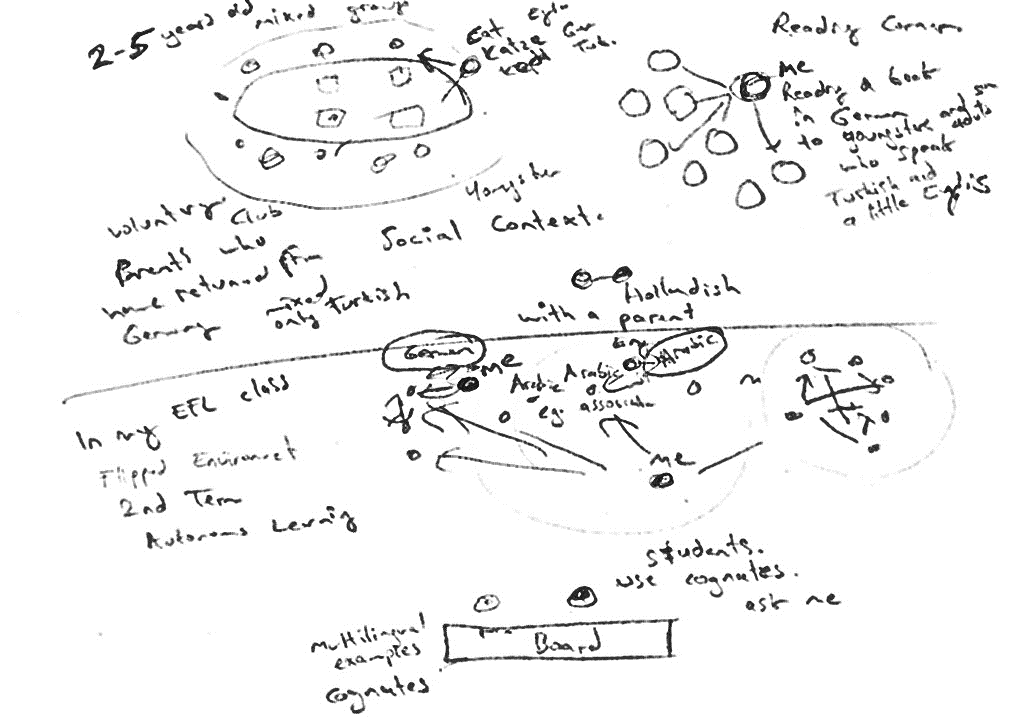
\includegraphics[width=.75\textwidth]{figures/a4-img001.png}
\caption{English teacher (TE)\label{fig:4:1}}
\end{figure}

\begin{figure}
\caption{German teacher (TG)\label{fig:4:2}}
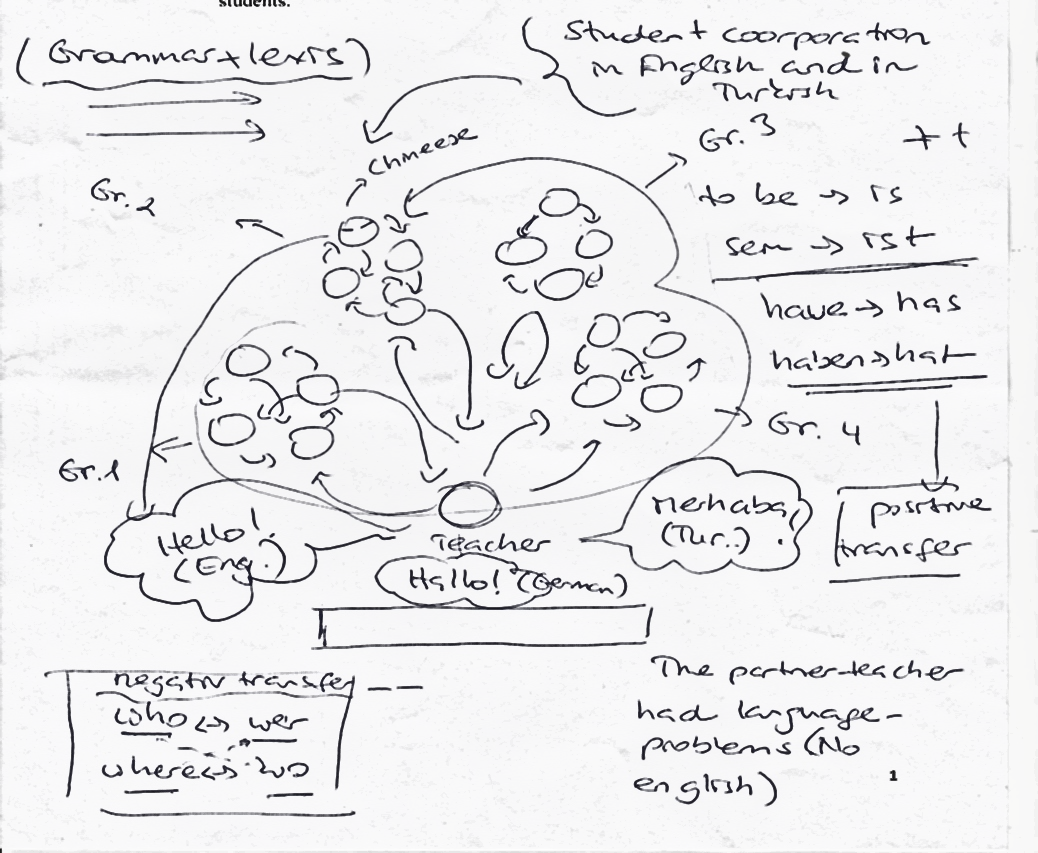
\includegraphics[width=.75\textwidth]{figures/a4-img002.png}
\end{figure}
  
\begin{figure}
\caption{Student 1 (SR1)\label{fig:4:3}}
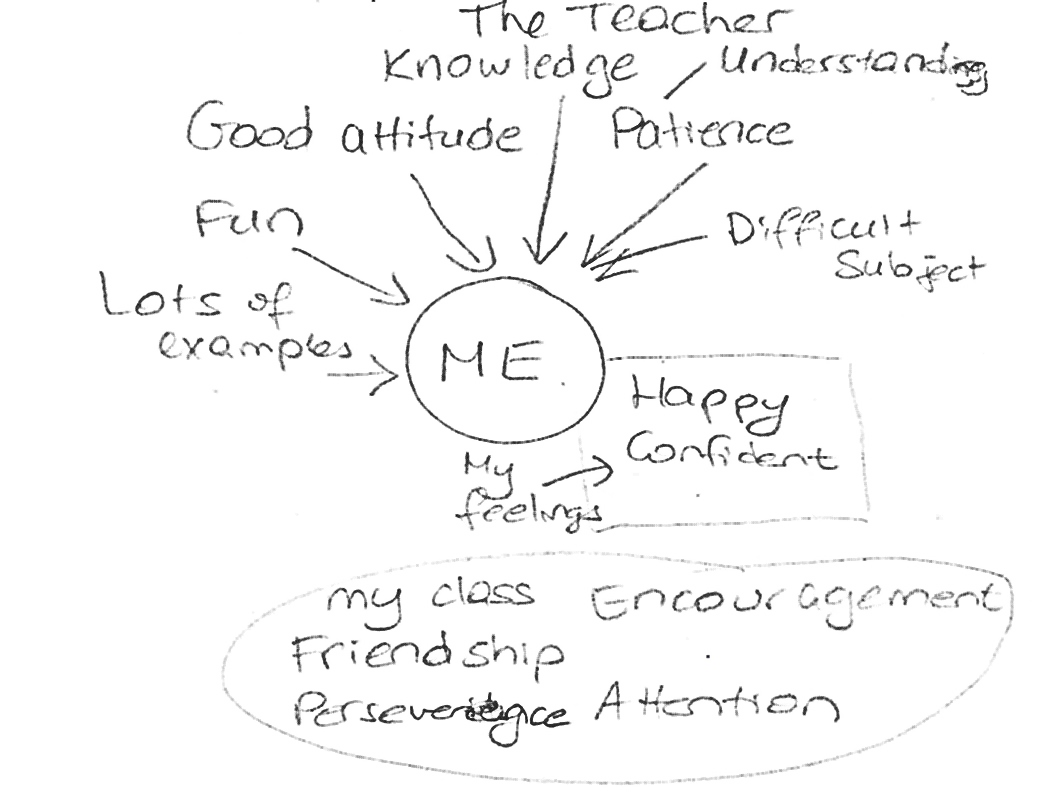
\includegraphics[width=.75\textwidth]{figures/a4-img003.png}
\end{figure}

\begin{figure}
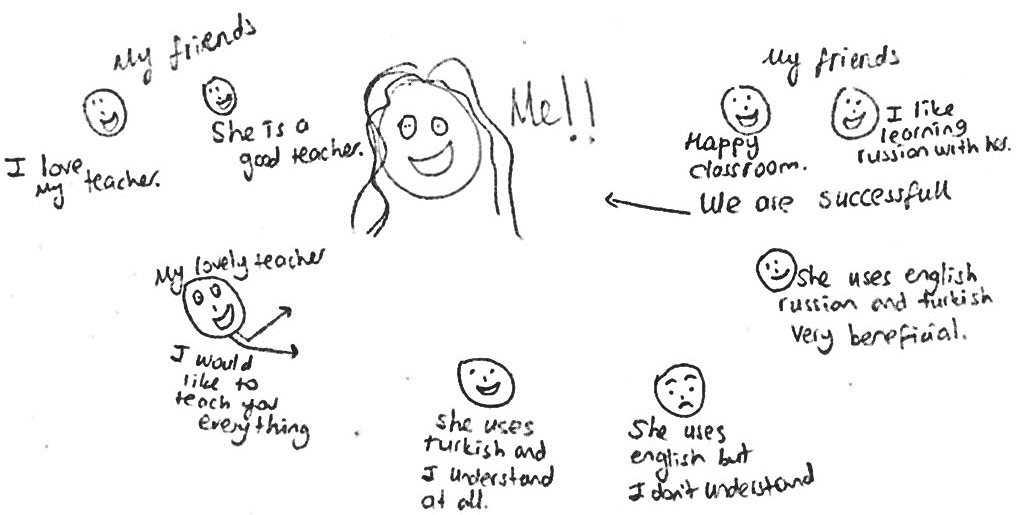
\includegraphics[width=.75\textwidth]{figures/a4-img004.png}
\caption{Student 2 (SR2)\label{fig:4:4}}
\end{figure}

{\sloppy\printbibliography[heading=subbibliography,notkeyword=this]}
\end{document}
